\chapter{الطاقة في الحياة اليومية}\label{ch:g5:everyday-energy}

لعبة ملفوفة تسرع على الأرض، ثم تبطئ، ثم تقف --- حتى تلفّها من
جديد. \omterm{def:g3:first-electric-circuit:bulb}{ومصباح} يدوي يخفت بينما تتعب بطاريتاه. وأنت نفسك ينفد نفَسك
قبل الغداء. فكل ما يتحرّك أو يضيء أو يُصوّت أو يُدفئ يبدو أنه
ينفق شيئًا. وللفيزياء اسم لذلك الشيء، ولعلّه أهمّ كلمة في هذا
الكتاب كله: \omterm{def:g5:everyday-energy:energy}{الطاقة}.

\section{الشيء الذي يُنجز الأمور}

\begin{definition}[الطاقة]\label{def:g5:everyday-energy:energy}
\emph{الطاقة}\index{طاقة} هي ما يلزم لكي تحدث الأشياء: لتحريكها،
ولرفعها، ولإضاءتها، ولتدفئتها، ولجعلها تُصوّت. فلا شيء يمضي أو
يتوهّج أو ينمو من غير أن تُنفَق عليه طاقة --- ومَن ينفق لا بدّ
أن يكون عنده أولًا طاقة ينفقها.
\end{definition}

\begin{definition}[مخازن الطاقة]\label{def:g5:everyday-energy:store}
\emph{مخزن الطاقة}\index{مخزن طاقة} كل ما يحمل \omterm{def:g5:everyday-energy:energy}{طاقة} مهيّأة
للاستعمال. والمخازن اليومية الكبرى: \emph{الغذاء} (وقود جسمك)،
و\emph{الوقود} مثل الحطب والبنزين، و\emph{البطاريات} المشحونة،
و\emph{النابض} الملفوف، والماء المحبوس \emph{عاليًا} خلف سدّ ---
و\emph{الشمس} الساخنة، تصبّ \omterm{def:g5:everyday-energy:energy}{الطاقة} على كل شيء طوال النهار،
مجّانًا.
\end{definition}

\begin{example}[اصطد المخزن]\label{ex:g5:everyday-energy:spot}
لكل شيء ماضٍ مخزن وراءه. فاللعبة المسرعة: نابضها الملفوف.
\omterm{def:g3:first-electric-circuit:bulb}{والمصباح} اليدوي: بطاريتاه. والسيارة: الوقود في خزّانها. وأنت:
فطورك. والقارب الشراعي: \omterm{def:g2:air-around-us:air}{الهواء} المتحرّك في \omterm{def:g2:air-around-us:wind}{الريح}. وحين يفرغ
المخزن --- فينفكّ النابض، وتنفد البطاريتان، ويجفّ الخزّان،
ويقترب موعد الغداء --- يتوقّف المضيّ.
\end{example}

\begin{remark}[لا مضيّ بلا تغذية]\label{rem:g5:everyday-energy:nofree}
طارد المخترعون قرونًا آلاتٍ تعمل إلى الأبد بلا شيء --- عجلات
تدير نفسها، وساعات لا تحتاج إلى لفّ. وفشلت كلها بلا استثناء
واحد. وفشلها من أعمق دروس الفيزياء: أن \omterm{def:g5:everyday-energy:energy}{الطاقة} لا تُستحضَر من
\omterm{def:g2:air-around-us:air}{هواء}. فكل ما يعمل يُغذَّى --- فجِد المخزن تفهم الآلة.
\end{remark}

\section{الطاقة تغيّر شكلها}

\begin{example}[أشكال الطاقة]\label{ex:g5:everyday-energy:forms}
تُظهر \omterm{def:g5:everyday-energy:energy}{الطاقة} نفسها في أشكال مختلفة: \omterm{def:g5:everyday-energy:energy}{طاقة} \emph{الحركة} في الكرة
المتدحرجة \omterm{def:g2:air-around-us:wind}{والريح} الهابّة؛ \omterm{def:g5:everyday-energy:energy}{وطاقة} \emph{\omterm{def:g1:light-and-shadows:source}{الضوء}} تنسكب من \omterm{def:g3:first-electric-circuit:bulb}{المصباح}
والشمس؛ \omterm{def:g5:everyday-energy:energy}{وطاقة} \emph{الحرارة} في كل ما هو دافئ؛ \omterm{def:g5:everyday-energy:energy}{والطاقة}
\emph{الكهربائية} تسافر في الأسلاك؛ \omterm{def:g5:everyday-energy:energy}{والطاقة} \emph{المخزونة}
تنتظر هادئة في الغذاء والوقود والنوابض والأشياء المرفوعة.
الشيء نفسه، وأشكال كثيرة.
\end{example}

\begin{proposition}[سلسلة الطاقة]\label{prop:g5:everyday-energy:chain}
كلما حدث شيء سُحبت \omterm{def:g5:everyday-energy:energy}{الطاقة} من مخزن ومُرّرت، وهي تغيّر شكلها في
الطريق عادةً. وهي لا تُخلق من لا شيء --- ولا تُفنى حقًّا أيضًا:
فما ``تستهلكه'' الآلة لم يفعل إلا أن مُرّر، وينتهي في الغالب،
عاجلًا أو آجلًا، دفئًا لطيفًا ينتشر في المحيط.
\end{proposition}

\begin{method}[كيف تقرأ سلسلة طاقة]\label{met:g5:everyday-energy:read}
لتفهم أي جهاز، تتبّع سلسلته:
\begin{enumerate}
  \item جِد \emph{المخزن} الذي تأتي منه \omterm{def:g5:everyday-energy:energy}{الطاقة}؛
  \item وجِد \emph{المحوِّل} --- أي الجزء الذي تغيّر فيه \omterm{def:g5:everyday-energy:energy}{الطاقة}
        شكلها؛
  \item وسمِّ الأشكال الخارجة --- النافع منها، والدفء المتسرّب
        إلى جانبه.
\end{enumerate}
\omterm{def:g3:first-electric-circuit:bulb}{والمصباح} اليدوي متتبَّعًا: \omterm{def:g3:first-electric-circuit:battery}{بطارية} (مخزن) $\to$ \omterm{def:g3:first-electric-circuit:bulb}{مصباح} (محوِّل)
$\to$ \omterm{def:g1:light-and-shadows:source}{ضوء} (نافع) $+$ قليل من الدفء (وهو التسرّب --- تحسّسه في
\omterm{def:g3:first-electric-circuit:bulb}{المصباح}).
\end{method}

\begin{omfigure}
\begin{tikzpicture}[scale=0.85]
  \node[draw, thick, omDef, font=\small, minimum width=2.5cm,
    minimum height=0.9cm] (a) at (1.4,0) {بطارية: مخزن};
  \node[draw, thick, omMeth, font=\small, minimum width=2.5cm,
    minimum height=0.9cm] (b) at (5.4,0) {مصباح: محوِّل};
  \node[draw, thick, omThm, font=\small, minimum width=2.2cm,
    minimum height=0.9cm] (c) at (9.4,0.7) {ضوء: نافع};
  \node[draw, thick, omExo, font=\small, minimum width=2.2cm,
    minimum height=0.9cm] (d) at (9.4,-0.7) {دفء: تسرّب};
  \draw[-Stealth, very thick] (a) -- (b);
  \draw[-Stealth, very thick] (b) -- (c);
  \draw[-Stealth, very thick] (b) -- (d);
\end{tikzpicture}

{\small سلسلة \omterm{def:g5:everyday-energy:energy}{طاقة} \omterm{def:g3:first-electric-circuit:bulb}{المصباح} اليدوي: \omterm{def:g5:everyday-energy:energy}{الطاقة} المخزونة تصير ضوءًا
--- وينسلّ قليل من الدفء إلى جانبه دائمًا.}
\end{omfigure}

\begin{example}[سلاسل في كل مكان]\label{ex:g5:everyday-energy:chains}
ركوبك الصباحي متتبَّعًا: فطور (مخزن) $\to$ عضلاتك (محوِّل)
$\to$ حركة الدرّاجة $+$ دفء (تحسّ به --- فأنت تتوهّج). ومزرعة
الرياح: \omterm{def:g2:air-around-us:air}{هواء} متحرّك $\to$ شفرات دائرة $\to$ \omterm{def:g5:everyday-energy:energy}{طاقة} كهربائية في
الأسلاك $\to$ \omterm{def:g1:light-and-shadows:source}{ضوء} في مصباحك الليلة. والسدّ: ماء عالٍ $\to$ ماء
ساقط يدير العنفات $\to$ \omterm{def:g5:everyday-energy:energy}{طاقة} كهربائية. وما السلاسل الطويلة إلا
قصيرات موصولة: شكل بعد شكل بعد شكل.
\end{example}

\begin{omfigure}
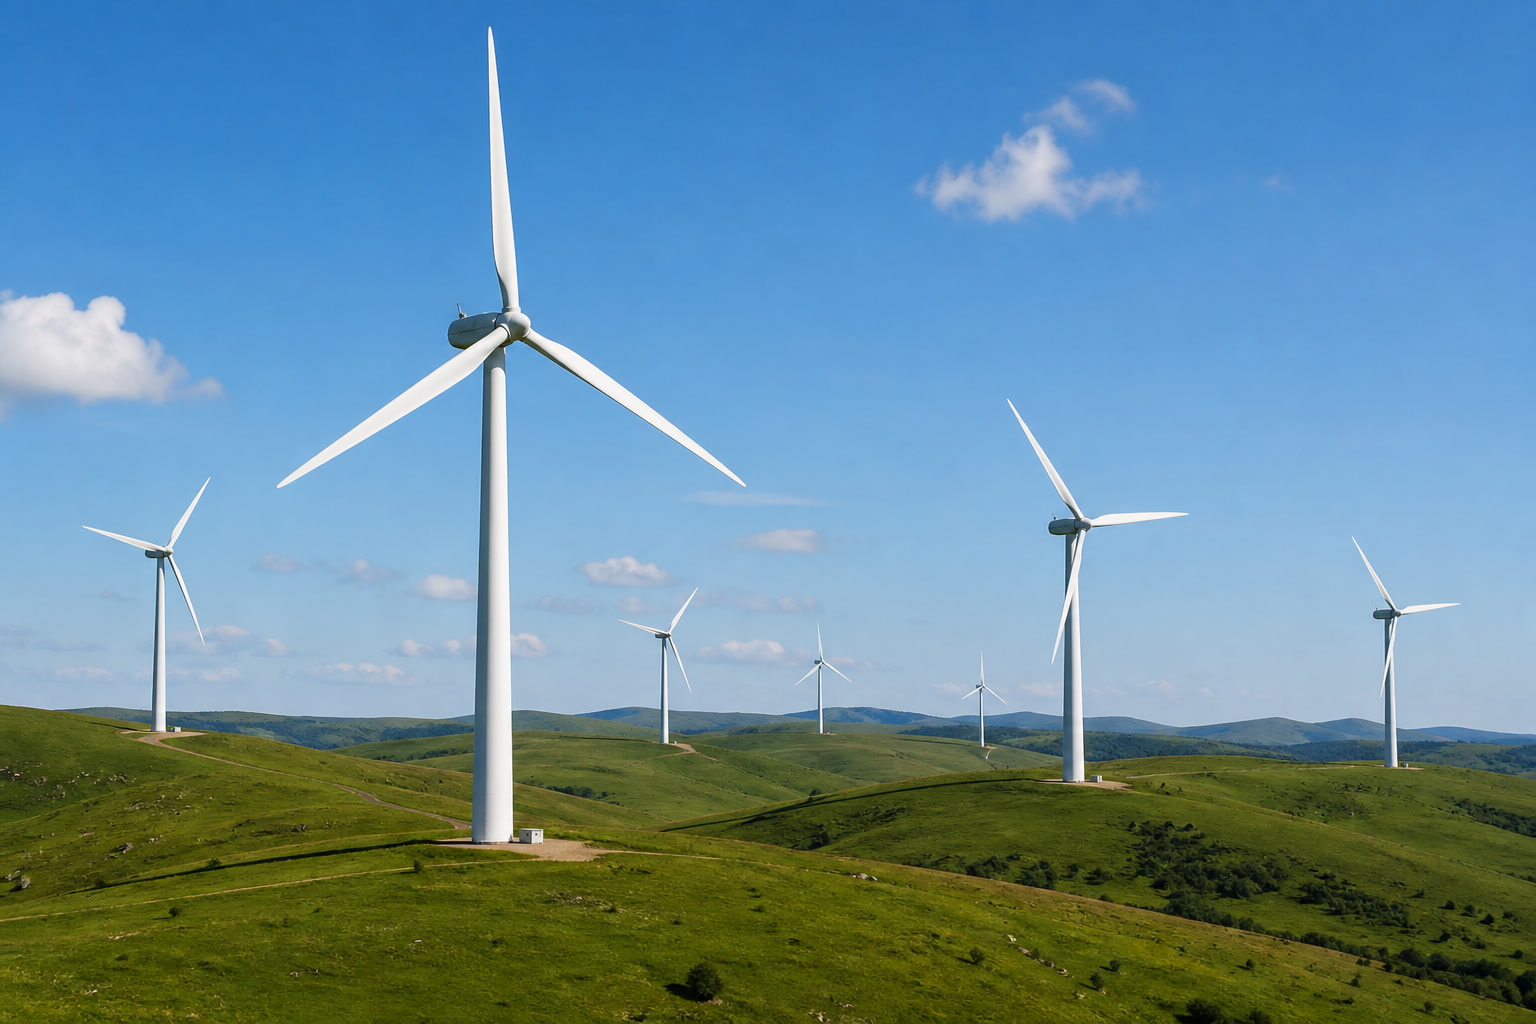
\includegraphics[width=0.58\linewidth]{images/book1/ai/g5-energy-windfarm.jpg}

{\small سلسلة \omterm{def:g5:everyday-energy:energy}{طاقة} تراها من الطريق: \omterm{def:g2:air-around-us:air}{هواء} متحرّك يدير الشفرات، فترسل العنفات \omterm{def:g5:everyday-energy:energy}{طاقة} كهربائية إلى الأسلاك.}
\end{omfigure}

\section{الشمس على رأس المائدة}

\begin{example}[أكثر السلاسل تبدأ عند الشمس]\label{ex:g5:everyday-energy:sun}
تتبّع أكثر السلاسل إلى الوراء تصل إلى الشمس. الفطور؟ أنبتته
نباتات التقطت \omterm{def:g1:light-and-shadows:source}{ضوء} الشمس؛ فحبوبك شمس معلَّبة. \omterm{def:g2:air-around-us:wind}{والريح}؟ الشمس تُدفئ
اليابسة على غير تساوٍ، \omterm{def:g2:air-around-us:air}{والهواء} المضطرب \omterm{def:g2:air-around-us:wind}{ريح} --- فحتى القوارب
الشراعية تعمل \omterm{def:g1:light-and-shadows:source}{بضوء} الشمس. والحطب؟ \omterm{def:g1:light-and-shadows:source}{ضوء} شمس خزّنته الأشجار. وماء
السدّ العالي؟ رفعته الشمس: بخّرت البحر، فأمطر البخار على
الجبال. أما الألواح الشمسية فتتخطّى الوسطاء لا غير.
\end{example}

\begin{omfigure}
\begin{tikzpicture}[scale=0.85]
  \fill[omThm] (0.9,3.2) circle (0.45);
  \foreach \a in {0,30,...,330} {
    \draw[omThm] (0.9,3.2) ++(\a:0.62) -- ++(\a:0.26);
  }
  \node[below, font=\small] at (0.9,2.5) {الشمس};
  \node[draw, thick, omMeth, font=\small] (p) at (4.3,3.2) {نباتات};
  \node[draw, thick, omDef, font=\small] (f) at (7.2,3.2) {غذاء};
  \node[draw, thick, omMeth, font=\small] (m) at (9.9,3.2) {عضلات};
  \node[draw, thick, omMeth, font=\small] (w) at (4.3,1.4)
    {هواء دافئ مضطرب};
  \node[draw, thick, omDef, font=\small] (v) at (8.3,1.4)
    {ريح وأشرعة};
  \draw[-Stealth, very thick] (1.6,3.2) -- (p);
  \draw[-Stealth, very thick] (p) -- (f);
  \draw[-Stealth, very thick] (f) -- (m);
  \draw[-Stealth, very thick] (1.35,2.75) -- (w);
  \draw[-Stealth, very thick] (w) -- (v);
\end{tikzpicture}

{\small سلسلتان متتبَّعتان إلى منبعهما: فالفطور \omterm{def:g2:air-around-us:wind}{والريح} كلاهما
يبدأ عند الشمس.}
\end{omfigure}

\begin{remark}[كلمة سنشحذها]\label{rem:g5:everyday-energy:promise}
\omterm{def:g5:everyday-energy:energy}{الطاقة} إلى الآن قصة حسنة الحكي: مخازن وأشكال وسلاسل. فهل يمكن
\emph{قياسها}، مثل الطول بالأمتار \omterm{def:g3:measuring-mass:mass}{والكتلة} بالغرامات؟ نعم ---
فللطاقة وحدتها الخاصة ودفترها الحسابي الدقيق، وهما يأتيان في
موضع لاحق من هذا الكتاب، بعد أن تلقى السرعة \omterm{def:g2:pushes-and-pulls:force}{والقوة} على أصولهما.
والسلاسل التي تتتبّعها هذه السنة هي الخريطة؛ وستأتي الأعداد
لتسكن فيها.
\end{remark}

\section{تمارين}

\begin{exercise}[$\star$]\label{exo:g5:everyday-energy:1}
ما \omterm{def:g5:everyday-energy:energy}{الطاقة}، بكلمات هذا الفصل؟ وسمِّ أربعة أشياء لا تحدث من
دونها.
\end{exercise}

\begin{exercise}[$\star$]\label{exo:g5:everyday-energy:2}
جِد المخزن: فأر ملفوف يسرع؛ \ راكب درّاجة؛ \ نار مخيّم؛
\ قارب شراعي؛ \ \omterm{def:g3:first-electric-circuit:bulb}{مصباح} يدوي.
\end{exercise}

\begin{exercise}[$\star$]\label{exo:g5:everyday-energy:3}
سمِّ خمسة أشكال \omterm{def:g5:everyday-energy:energy}{للطاقة}، مع مثال واحد لكل شكل من
يومك أنت.
\end{exercise}

\begin{exercise}[$\star$]\label{exo:g5:everyday-energy:4}
تتبّع سلسلة \omterm{def:g5:everyday-energy:energy}{طاقة} محمصة الخبز، كما في
\cref{met:g5:everyday-energy:read}: مخزن، ومحوِّل، وأشكال
خارجة.
\end{exercise}

\begin{exercise}[$\star$]\label{exo:g5:everyday-energy:5}
تتبّع السلسلة من بحيرة سدّ إلى \omterm{def:g3:first-electric-circuit:bulb}{مصباح} قراءتك الليلة.
\end{exercise}

\begin{exercise}[$\star$]\label{exo:g5:everyday-energy:6}
هاتف ``يموت''. فما الذي نفد حقًّا؟ وإلى أين ذهبت تلك \omterm{def:g5:everyday-energy:energy}{الطاقة}،
وفق قضية السلسلة؟
\end{exercise}

\begin{exercise}[$\star$]\label{exo:g5:everyday-energy:7}
لماذا يسخن الحاسوب المحمول من تحت وأنت تستعمله؟ وأيّ حلقة من
حلقات السلسلة تُظهر نفسها؟
\end{exercise}

\begin{exercise}[$\star$]\label{exo:g5:everyday-energy:8}
بيّن أن القارب الشراعي يعمل \omterm{def:g1:light-and-shadows:source}{بضوء} الشمس، بتتبّع سلسلته إلى
الوراء خطوة خطوة.
\end{exercise}

\begin{exercise}[$\star\star$]\label{exo:g5:everyday-energy:9}
يعلن مخترع عن \omterm{def:g3:first-electric-circuit:bulb}{مصباح} ``لا يحتاج إلى \omterm{def:g3:first-electric-circuit:battery}{بطارية} ولا قابس ولا وقود ---
إنما يضيء إلى الأبد''. فأيّ درس من
\cref{rem:g5:everyday-energy:nofree} يتحدّاه هذا الإعلان؟ وأيّ
سؤال ينبغي أن تسأل المخترعَ أولًا؟
\end{exercise}

\begin{exercise}[$\star\star$]\label{exo:g5:everyday-energy:10}
كرة مطّاطية تُسقط من ارتفاع الكتف ترتدّ أدنى فأدنى ثم تستقرّ
ساكنة أخيرًا. يقول ليو: ``فنيت طاقتها.'' استعمل
\cref{prop:g5:everyday-energy:chain} للدفاع عن نهاية أفضل
للقصة --- إلى أيّ شكل نهائي انسلّت \omterm{def:g5:everyday-energy:energy}{طاقة} الارتداد؟
\end{exercise}

\begin{exercise}[$\star\star$]\label{exo:g5:everyday-energy:11}
بعض البيوت تسخّن الماء في ألواح سوداء على السطح؛ وبعضها يطبخ
\omterm{def:g1:light-and-shadows:source}{بضوء} الشمس ومرايا مقعّرة؛ والخلايا الشمسية تصنع كهرباء من \omterm{def:g1:light-and-shadows:source}{ضوء}
النهار. اشرح عبارة ``الألواح الشمسية تتخطّى الوسطاء لا غير'' في
\cref{ex:g5:everyday-energy:sun}: مَن الوسطاء الواقفون بين
الشمس ودفء نار الحطب؟
\end{exercise}
